%-------------------------------------------------------------------------------

% This file is part of Code_Saturne, a general-purpose CFD tool.
%
% Copyright (C) 1998-2013 EDF S.A.
%
% This program is free software; you can redistribute it and/or modify it under
% the terms of the GNU General Public License as published by the Free Software
% Foundation; either version 2 of the License, or (at your option) any later
% version.
%
% This program is distributed in the hope that it will be useful, but WITHOUT
% ANY WARRANTY; without even the implied warranty of MERCHANTABILITY or FITNESS
% FOR A PARTICULAR PURPOSE.  See the GNU General Public License for more
% details.
%
% You should have received a copy of the GNU General Public License along with
% this program; if not, write to the Free Software Foundation, Inc., 51 Franklin
% Street, Fifth Floor, Boston, MA 02110-1301, USA.

%-------------------------------------------------------------------------------

%-------------------------------------------------------------------------------
\section{Introduction}

%-------------------------------------------------------------------------------
\subsection{Definition and notations}\label{sec:spadis:notations}

Within the framework of the finite volume approach, the equations are
integrated over each cell of the mesh (or \emph{control volume} $\vol{\celli}$). 
\nomenclature[gomegai]{$\vol{\celli}$}{the cell $\celli$}
This section is limited to a brief description of the way $0^{th}$-order, convection, diffusion and gradient terms appearing in
the equations are integrated using the budget methodology. Specific attention is devoted to the
calculation of gradients, since it is a major characteristic of the
co-located finite volume method (all the variables are associated with the
same point, namely the cell centre\footnote{%
The centre of a cell is a geometric point associated with the cell and
located preferably inside the cell. Nevertheless, the word \emph{centre} shall
not be taken literally,
especially in the case of polyhedral cells that do not have a regular shape.}%
).

Let $\ncell$ be the number of cells, then each discretized field $\varia$ has $\ncell$ degrees of freedom,
which are denoted by $\varia_\celli$, $\celli \in \left[ 1 , \, \cdots , \, \ncell \right]$ given by definition by:
\begin{equation}\label{eq:spadis:variai_def}
\varia_\celli \equiv \dfrac{1}{\norm{\vol{\celli}}}\int_{\vol{\celli}} \varia \dd \vol{}.
\end{equation}

As each discretized field $\varia$ is supposed to be linear in every single cell, $\varia_\celli$ can be identified
by the value of the field in $\centi$, the cell center of $\vol{\celli}$:
\begin{equation}\label{eq:spadis:variai_id}
\varia_\centi = \varia_\celli.
\end{equation}

%-------------------------
\paragraph{$0^{th}$-order terms:}
Then, terms of \textbf{order $0$} (\emph{i.e.} terms that are not space
derivatives) are integrated to introduce their average over the cell. For
example, $\rho \vect{g}$ becomes $\norm{\vol{\celli}} \rho_{\celli} \vect{g}$. 
\nomenclature[gomegaiv]{$\norm{\vol{\celli}}$}{volume of the cell $\celli$ \nomunit{$m^{3}$}}
In this expression, $\norm{\vol{\celli}}$ is the measure of cell volume $\vol{\celli}$ and 
$\rho_{\celli}$ denotes the average of $\rho $ over the control volume
(the cell) $\vol{\celli}$ applying \eqref{eq:spadis:variai_def}. 
\nomenclature[riu]{$\centi$}{centre of $\vol{\celli}$}

%-----------------------------------------
\paragraph{Divergence operator--conservative gradient terms:}
The \textbf{divergence} terms (or \emph{flux} terms, or again \emph{conservative}
terms) are integrated using the Green relation to introduce cell faces
values so that \emph{fluxes} appear naturally. For example, a term such as 
$\divv \left( \varia \tens{1}\right)$ becomes\footnote{%
in $\divv \left( \varia \tens{1}\right)$, $\varia$ might be the pressure field $P$, this term then corresponds to the pressure gradient
in the momentum equation.
}%

%\footnote{%
%If the cell $\celli$ is at the domain boundary, the sum becomes 
%$\sum\limits_{\fij \in \Facei{\celli}} P_{\fij} \vect{S}_{\ij}+\sum\limits_{\fib \in \Faceb{\celli}} P_{\fib} \vect{S}_{\ib}$, 
%with $\fib$ referring to the faces
%of the cell $\celli$ which are at the domain boundary.
%} %

\begin{equation}\label{eq:spadis:green_relation}
\int_{\vol{\celli}} \divv \left( \varia \tens{1}\right) \dd \vol{} =  \sum\limits_{\face \in \Face{\celli}} \varia_{\face}\vect{S}_{\iface}.
\end{equation}
\nomenclature[rface]{$\face$}{interior or boundary cell face \nomunit{}}
\nomenclature[rfacei]{$\Face{\celli}$}{group of all faces of the cell $\celli$ \nomunit{}}
\nomenclature[rsifacei]{$\vect{S}_{\iface}$}{outward normal vector of the face $\face$ of the cell $\celli$, normalized by the surface $\norm{\vect{S}}$  \nomunit{}}

In expression \eqref{eq:spadis:green_relation}, face values of the field $\varia$ appear. They are defined as:
\begin{equation}\label{eq:spadis:variaf_def}
\varia_\face \equiv \dfrac{1}{\norm{\vect{S}}_\face} \int_{\face} \varia \dd S,
\end{equation}
%
so that the relationship \eqref{eq:spadis:green_relation} is exact. As the field $\varia$ is linear over the face $\face$,  
$\varia_\face$ can be associated to the face centre $\centf$:
\begin{equation}\label{eq:spadis:variaf_id}
\varia_\centf = \varia_\face.
\end{equation}

In the following sections, faces $\Face{\celli}$ are usually split into two categories: the interior faces $\fij \in \Facei{\celli}$ separating
two neighbouring cells $\celli$ and $\cellj$; and the boundary faces $\fib \in \Faceb{\celli}$. 
Outward (with respect to the cell $\celli$) normals are respectively denoted  $\vect{S}_\ij$ and $\vect{S}_\ib$, 
which means that $\vect{S}_\ij$ is oriented from $\celli$ toward $\cellj$. 

Then $\varia_{\centf}$ is expressed as an average of the degree of freedom, which are for the interface $\fij$ the value of $\varia_\celli$ 
and $\varia_\cellj$ but also the gradients in these cells. The use of gradients to reach an higher order in space is called \emph{reconstruction} 
in the coming sections. The detailed computation of $\int_{\vol{\celli}} \divv \left( \varia \tens{1}\right) \dd \Omega $ is given in
 \S~\ref{sec:spadis:iteratif_gradient}. 
%
\nomenclature[rpij]{$P_{\fij}$}{average of the pressure field on the interface between the neighbouring cells $\celli$ and $\cellj$ \nomunit{$Pa$}}
\nomenclature[rfu]{$\centf$}{center of the face $\fij$ between cells $\celli$ and $\cellj$}
 
 %-----------------------------------------------
\paragraph{Convection operator--mass flux terms:}
 Let us now focus on the convective term $\dive \left( \varia \rho \vect{u}\right)$. This term and the
 non-stationary term $ \der{ \left( \rho \varia \right) }{ t} $ will be treated
 together. As a matter of fact, if the field $\varia$ is transported by the convective field $\rho \vect{u}$, the balance
 of the quantity $\rho \varia$ over a cell $\celli$ is written using Leibniz theorem as:
 %
 \begin{equation}\label{eq:spadis:leibnitz_th}
\begin{array}{r c l}
\displaystyle \DP{} \left( \int_{\vol{\celli}} \rho \varia \dd \vol{}\right) &=& 
\displaystyle \int_{\vol{\celli}} \der{\rho \varia}{t} \dd \vol{} + \int_{\partial \vol{\celli}} \varia \rho \vect{u} \cdot  \dd \vect{S}, \\
\displaystyle &=&
\displaystyle \int_{\vol{\celli}} \der{\rho \varia}{t} + \dive \left( \varia \rho \vect{u} \right)  \dd \vol{},
\end{array}
 \end{equation}
the second line is obtained using Green relation. 
 
Moreover, the non-stationary and convection terms are usually written in a \emph{non-conservative} form that is in continuous formalism:
\begin{equation}\label{eq:spadis:non_conservative}
 \der{ \left( \rho\varia \right)}{t} + \dive \left(  \varia  \rho \vect{u}\right) = \rho \der{\varia }{t} + \grad \varia \cdot \left( \rho \vect{u}\right) + \Gamma \varia.
 \end{equation}
 Note that for \eqref{eq:spadis:non_conservative} to hold, the continuity equation \eqref{eq:mass} must be fulfilled. 
 If \eqref{eq:spadis:non_conservative} is required even for discrete volumes, the convection term must be defined as:
 %
 \begin{equation}\label{eq:spadis:convection_def}
 \begin{array}{r c l}
\displaystyle \int_{\vol{\celli}} \grad \varia \cdot \left( \rho \vect{u} \right) \dd \vol{} &\equiv &
\displaystyle \int_{\vol{\celli}}  \dive \left( \varia \rho \vect{u} \right) \dd \vol{}  - \varia_\celli  \int_{\vol{\celli}} \dive \left(\rho \vect{u} \right) \dd \vol{}, \\
 &=& 
 \displaystyle \int_{ \partial \vol{\celli}}   \varia \rho \vect{u} \cdot \dd \vect{S}  - \varia_\celli  \int_{ \partial \vol{\celli}} \rho \vect{u} \cdot \dd \vect{S}, \\
 &=& 
\displaystyle \sum_{\face \in \Face{\celli}} \left(\varia_\face - \varia_\celli \right) \left(\rho \vect{u}\right)_\face \cdot \vect{S}_{\iface},
 \end{array}
 \end{equation}
the second line is obtained using once again Green relation. In formula \eqref{eq:spadis:convection_def}, one still has to express the face value
 $\varia_\face$ and also the value of the mass flux $\left(\rho \vect{u}\right)_\face\cdot \vect{S}_{\iface}$: all the available convective schemes (\emph{upwind, centred, SOLU, etc.}) are presented in \S~\ref{sec:spadis:convection}. Let $\dot{m}_\iface$ be the outgoing
 mass flux from cell $\celli$ through the face $\face$:
 %
  \begin{equation}\label{eq:spadis:massflux_def}
\dot{m}_\iface \equiv \left(\rho \vect{u}\right)_\face \cdot \vect{S}_{\iface},
 \end{equation}
note that this convective flux is naturally defined at cell faces and thus is stored over there in the code. In the following, the convection term is denoted as follows:
\begin{equation}\label{eq:spadis:convection_notation}
\displaystyle \int_{\vol{\celli}} \grad \varia \cdot \left( \rho \vect{u} \right) \dd \vol{} 
=
\displaystyle \sum_{\face \in \Face{\celli}} C_\iface \left( \dot{m}_\iface , \, \varia \right),
 \end{equation}
where $C_\iface \left(  \dot{m}_\iface  , \, \varia\right)$ is defined by:
\begin{equation}\label{eq:spadis:convection_flux}
C_\iface \left(\dot{m}_\face , \, \varia \right) \equiv  \left(\varia_\face - \varia_\celli \right) \dot{m}_\iface.
 \end{equation}

 %----------------------------------------------
\paragraph{Laplacian operator--diffusive terms:}
Let us discretize the diffusive term $\dive \left(  K \grad \varia  \right) $:
%
 \begin{equation}\label{eq:spadis:diffusion_def}
 \begin{array}{r c l}
\displaystyle \int_{\vol{\celli}} \dive \left( K \grad \varia\right) \dd \vol{} &\equiv &
\displaystyle \sum_{\face \in \Face{\celli}} K_\face \grad_\face \varia \cdot \vect{S}_{\iface},
 \end{array}
 \end{equation}
  where $K_\face$ is the face diffusivity, and $\grad_\face \varia$ is the face gradient, their computation will be detailed in \S~\ref{sec:spadis:diffusion}. In the following, the diffusive term is denoted as follows:
  %
\begin{equation}\label{eq:spadis:diffusion_notation}
\int_{\vol{\celli}} \dive \left( K \grad \varia\right) \dd \vol{} 
 =
\sum_{\face \in \Face{\celli}} D_\iface \left(  K_\face \,  \varia \right),
\end{equation}    
 where the diffusive flux $D_\iface \left(  K_\face \,  \varia \right)$ over the face $\face$ is defined by:
 \begin{equation}\label{eq:spadis:diffusion_flux}
D_\iface \left( K_\face , \, \varia\right) \equiv   K_\face \grad_\face \varia \cdot \vect{S}_{\iface}.
 \end{equation}
 Note that the diffusive flux $D_\ij \left( K_\fij , \, \varia\right) $ over the interior face $\fij$ lost by the cell $\celli$
 is gained by $\cellj$, in other words:
 \begin{equation}\label{eq:spadis:diffusion_flux_symmetry}
D_\ij \left( K_\fij , \, \varia\right) = - D_\ji \left( K_\fij , \, \varia\right) .
 \end{equation} 
 
 \begin{remark}
The diffusion operator can be extended to anisotropic tensor diffusivity $\tens{K}$.
 \end{remark}
 
 %---------------------------------------
 \paragraph{More geometrical quantities:}
To end up the general description of the discretized operators, let us introduce some geometrical 
quantities which will be used during the approximation process of linking face fluxes to 
cell centred quantities. 
% fa modification : reconstruction is compulsory for consistence
For consistency and to reach a higher order in space, the values of the
variables at points $\centip$ and $\centjp$ have to be used. 
These points are respectively the projection of the centres $\centi$ and $\centj$ 
along the orthogonal line to the interior face $\fij$ passing through $\centf$. 
When considering a boundary face $\fib$, $\centip$ is defined as the projection of $\centi$
on the normal to the boundary face $\fib$ passing through $\centf$. All the geometrical
definitions are recalled in \figurename~\ref{fig:sketch_internal_external_faces}.
%
Using Taylor series from the values at $\centi$ and $\centj$ and from the \emph{cell gradient}
in the respective cells, one can write for any field $\varia$:
\begin{equation}\label{eq:spadis:reconstruction_ip_jp}
\left\lbrace
\begin{array}{r c l c l}
\varia_\centip &\simeq & \varia_\centi + \grad_\celli \varia \cdot \vect{\centi \centip} &=& \varia_\celli + \grad_\celli \varia \cdot \vect{\centi \centip},  \\
\varia_\centjp &\simeq & \varia_\centj + \grad_\cellj \varia \cdot \vect{\centj \centjp} & =& \varia_\cellj + \grad_\cellj \varia \cdot \vect{\centj \centjp}. 
\end{array}
\right.
\end{equation}
Note that for orthogonal meshes (where $\centip = \centi$ for all faces of all cells), 
no \emph{reconstruction} \eqref{eq:spadis:reconstruction_ip_jp} is needed, 
and therefore the distance $\norm{\vect{\centi \centip}}$ measures the \emph{non-orthogonality} of the mesh.
The computation of $\grad_\celli \varia$ is presented in  \S~\ref{sec:spadis:iteratif_gradient} and \S~\ref{ap:gradrc}.

Furthermore, the intersection between \vect{\centi \centj} and the corresponding interior face $\fij$ is denoted by $\cento$. 
The distance $\norm{\vect{\cento \centf}}$ measures the \emph{offset} of the mesh. 

Eventually, a weighting factor $\alpha_\ij$ is defined to measure the distance of the cell center $\centi$ to the face $\fij$ relatively 
to the other cell center $\centj$:
\begin{equation}\label{eq:spadis:pond_def}
\alpha_{\ij}=\dfrac{\overline{\centf \centjp}}{\overline{\centip \centjp}}.
\end{equation}
Note that the distances  $\overline{\centip \centjp}$ and $\overline{\centf \centjp}$ are defined algebraically, that is:
\begin{equation}
\begin{array}{r c l}
\overline{\centip \centjp} & \equiv & \dfrac{\vect{\centip \centjp} \cdot \vect{S}_\ij}{\norm{\vect{S}_\ij}}, \\
\overline{\centf \centjp} & \equiv & \dfrac{\vect{\centf \centjp} \cdot \vect{S}_\ij}{\norm{\vect{S}_\ij}},
\end{array}
\end{equation}
and are supposed to be positive if the mesh is \emph{star-shaped}. Note also that $\alpha_\ij$ is oriented from $\celli$ to $\cellj$ and 
%
\begin{equation}
\alpha_\ij + \alpha_\ji = 1.
\end{equation}

\begin{figure}[t]
\centering
\mbox{
\subfigure[Internal face]{
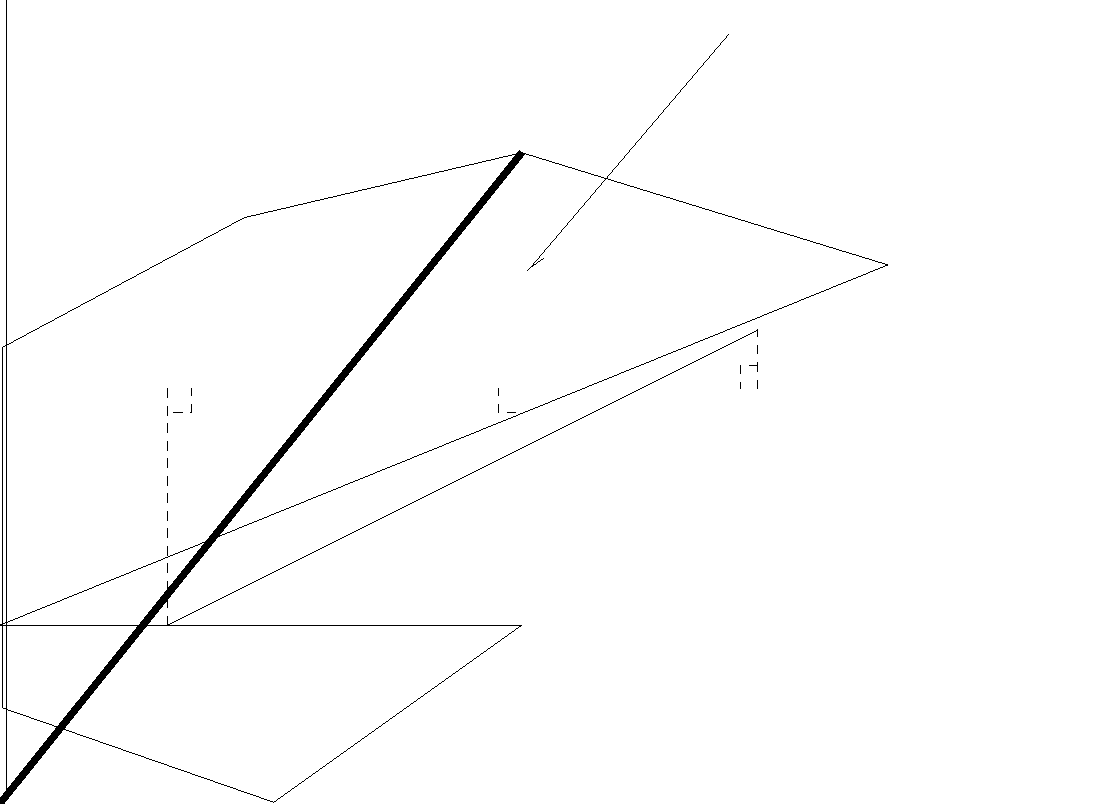
\includegraphics[width=0.45 \textwidth]{facette}
} \,
\subfigure[Boundary face]{
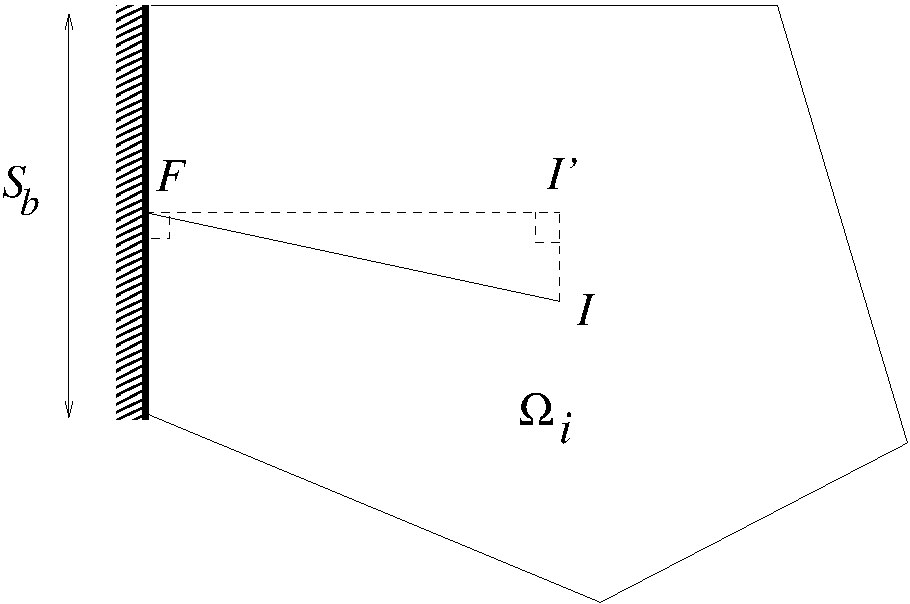
\includegraphics[width=0.45 \textwidth]{facebord}
}
}%end mbox
\caption{Sketch of geometric entities.}
\label{fig:sketch_internal_external_faces}
\end{figure}


%-------------------------------------------------------------------------------
\section{Convective term}\label{sec:spadis:convection}
Using the notations adopted in \S~\ref{sec:spadis:notations}, 
the explicit budget corresponding to the integration over a cell
$\vol{\celli}$ of the convective part $\grad_\celli \varia \cdot \left(\rho \vect{u} \right) $
has been written as a sum of the
numerical fluxes $C_\ij \left( \dot{m}_\ij , \, \varia \right)$ calculated at the interior faces,
 and the numerical fluxes $C_\ib \left( \dot{m}_\ib , \, \varia \right)$ calculated at the
boundary faces of the computational domain $\Omega$ defined by Equation~\eqref{eq:spadis:convection_flux}.

Note that $C_\ib \left( \dot{m}_\ib , \, \varia \right)$ makes appear the boundary conditions of the field $\varia$
 and are described in detail in \chaptername~\ref{chapter:bndcnd}. The value of $\varia_\fib$ is expressed as follows:
 %
\begin{equation}%TODO use recall
\varia_\fib \equiv A_\fib^g + B_\fib^g \varia_\centip.
\end{equation}


The value of the convective flux $ C_\ij \left(\dot{m}_\fij , \, \varia \right) $ depends on the numerical scheme. Three different types of convection schemes are available in \CS.

%-------------------------------------------------------------------------------
\subsection{Upwind}
For a $1^{st}$-order upwind scheme, the convective flux reads:

\begin{equation}
C_\ij^{upwind} \left( \dot{m}_\ij , \, \varia \right)  \equiv \left(\varia_\fij^{upwind} - \varia_\celli \right) \dot{m}_\ij, 
\end{equation}
with
\begin{equation}
\varia_\fij^{upwind} = 
\left\lbrace\begin{array}{l}
\varia_\celli \text{ if } \dot{m}_\ij  \geqslant 0,\\
\varia_\cellj \text{ if } \dot{m}_\ij < 0.
\end{array}\right. 
\end{equation}


%-------------------------------------------------------------------------------
\subsection{Centred}
For a centred scheme, the convective flux reads:

\begin{equation}
C_\ij^{centred} \left( \dot{m}_\ij , \, \varia \right)  \equiv \left(\varia_\fij^{centred} - \varia_\celli \right) \dot{m}_\ij ,
\end{equation}
with
\begin{equation}
\varia_\fij^{centred} = \alpha_\ij \varia_\centip + \left( 1 - \alpha_\ij \right) \varia_\centjp.
\end{equation}

\begin{remark}

We actually write
%
\begin{equation}
\varia_\fij^{centred} = \alpha_\ij \varia_\celli + \left( 1 - \alpha_\ij \right) \varia_\cellj
+
\dfrac{1}{2} \left[ \grad_\celli \varia + \grad_\cellj \varia \right] \cdot \vect{OF},
\end{equation}
%
which ensures the first-order discretization in space for $\varia$.  
The factor $ \frac{1}{2}$ is used for numerical stability reasons.
\end{remark}

%-------------------------------------------------------------------------------
\subsection{Second Order Linear Upwind (SOLU)}
For a $2^{nd}$-order linear upwind scheme\footnotetext{%
Extrapolation  of the upwind value at the faces centre.}%
, the convective flux reads:

\begin{equation}
C_\ij^{SOLU} \left( \dot{m}_\ij , \, \varia \right)  \equiv \left(\varia_\fij^{SOLU} - \varia_\celli \right) \dot{m}_\ij ,
\end{equation}
with
\begin{equation}
\varia_\fij^{SOLU} =
\left\lbrace\begin{array}{l l}
\varia_\celli +\grad_\celli \varia \cdot \vect{IF}  & \text{ if }  \varia_\celli \text{ if } \dot{m}_\ij  \geqslant 0,\\
\varia_\cellj +\grad_\cellj \varia \cdot\vect{JF}   & \text{ if } \varia_\cellj \text{ if } \dot{m}_\ij < 0 .
\end{array}\right.
\end{equation}


The value of $C_\ib^{SOLU}$ is calculated as:
\begin{equation}
\varia_\fib^{SOLU} =
\left\lbrace\begin{array}{l l}
\varia_\celli +\grad_\celli \varia \cdot \vect{IF}  &\text{ if }  \varia_\celli \text{ if } \dot{m}_\ib  \geqslant 0,\\
A^g_\fib  + B^g_\fib \varia_\centip  & \text{ if } \varia_\cellj \text{ if } \dot{m}_\ij < 0.
\end{array}\right.
\end{equation}

\begin{remark}
A slope test (which may introduce non-linearities in the convection operator) allows to switch from 
the centred or SOLU scheme to the first-order upwind scheme (without blending). Additionally, the default option to deal with $\varia_\fij$ is 
computed as a weighted average between the upstream value and the centred value (blending), according to users' choice.
\end{remark}


%-------------------------------------------------------------------------------
\section{Diffusive term}\label{sec:spadis:diffusion}
Using the notations adopted in \S~\ref{sec:spadis:notations}, 
the explicit budget corresponding to the integration over a cell
$\vol{\celli}$ of the diffusive term $\dive \left( K \grad \varia \right) $
has been written as a sum of the
numerical fluxes $D_\ij \left( K_\fij , \, \varia \right)$ calculated at the internal faces,
 and the numerical fluxes $D_\ib \left( K_\fib , \, \varia \right)$ calculated at the
boundary faces of the computational domain $\Omega$ defined by Equation~\eqref{eq:spadis:diffusion_flux}.

Note that $D_\ib \left( K_\fib , \, \varia \right)$ makes appear the \textbf{diffusion} boundary conditions of the field $\varia$
 and are described in detail in \chaptername~\ref{chapter:bndcnd}. The value of flux $D_\ib $ of the $\varia_\fib$ is expressed as follows:
 %
\begin{equation}\label{eq:spadis:boundary_flux}%TODO use recall
\dfrac{D_\ib}{\norm{\vect{S}}_\fib}  \equiv A_\ib^f + B_\ib^f \varia_\centip.
\end{equation}

The value of the diffusive flux $D_\ij $ depends on the \emph{reconstruction} of the field $\varia$ and also on the interpolation at the face  of the diffusivity $K$ from the cell values. Two interpolations are available:
%
\begin{enumerate}[ label=\roman{*}/, ref=(\roman{*})]
\item a \emph{harmonic} interpolation which reads:
\begin{equation}\label{eq:spadis:harmonic_viscosity}
K_\fij^{harmonic} \equiv  \dfrac{K_\celli K_\cellj}{\alpha_\ij K_\celli + \left( 1 - \alpha_\ij\right)K_\cellj}
\end{equation}
\item an \emph{arithmetic} interpolation which reads:
\begin{equation}
K_\fij^{arithmetic} \equiv  \dfrac{1}{2} \left( K_\celli + K_\cellj\right)
\end{equation}
\end{enumerate}
Note that to ensure flux continuity at the internal faces $\fij$, one should use the \emph{harmonic} mean, 
whereas the \emph{arithmetic} mean is set as the default option because it has been proven to be more robust numerically.

%-------------------------------------------------------------------------------
\subsection{Without reconstruction}
For a \emph{non-reconstructed} field, the diffusive flux reads:

\begin{equation}
D_\ij^{NRec} \left( K_\fij , \, \varia \right)  =  - \dfrac{K_\fij \norm{\vect{S}_\ij}}{\overline{\centip \centjp} } \left( \varia_\celli - \varia_\cellj\right).
\end{equation}


%-------------------------------------------------------------------------------
\subsection{Reconstructed}
For a \emph{reconstructed} field, the diffusive flux reads:

\begin{equation}
D_\ij^{Rec} \left( K_\fij , \, \varia \right)  =  - \dfrac{K_\fij \norm{\vect{S}_\ij}}{\overline{\centip \centjp} } \left( \varia_\centip - \varia_\centjp \right).
\end{equation}

\begin{remark}
In fact, it is actually written that
%
\begin{equation}
\begin{array}{r c l}
D_\ij^{Rec} \left( K_\fij , \, \varia \right)  &=&  - \dfrac{K_\fij \norm{\vect{S}_\ij}}{\overline{\centip \centjp} } \left( \varia_\celli - \varia_\cellj \right) \\
&-& \dfrac{K_\fij \norm{\vect{S}_\ij}}{\overline{\centip \centjp} }  \dfrac{1}{2}\left( \grad_\celli \varia + \grad_\cellj \varia \right) \cdot \left( \vect{\centi \centip} - \vect{\centj \centjp} \right),
\end{array}
\end{equation}
%
which ensures the first-order discretization in space for $\varia$.  
The factor $ \frac{1}{2}$ is used for numerical stability reasons.
\end{remark}


%-------------------------------------------------------------------------------
\section{Gradient calculation}

The aim of the present section is to describe the algorithms available in \CS 
to compute cell gradient for scalar or vector fields. The first one uses an 
iterative process to handle with non-orthogonalities. It is robust but requires 
computational effort. The second one, the least square method, minimizes a 
function. It is quick, but less accurate.

For both methods, the adaptation to gradients of vectorial fields is also presented.

%-------------------------------------------------------------------------------
\subsection{Standard method: iterative process}\label{sec:spadis:iteratif_gradient}


\subsubsection{General description}
\begin{figure}[!htbcp]
\centering
\mbox{
\subfigure[Internal face]{
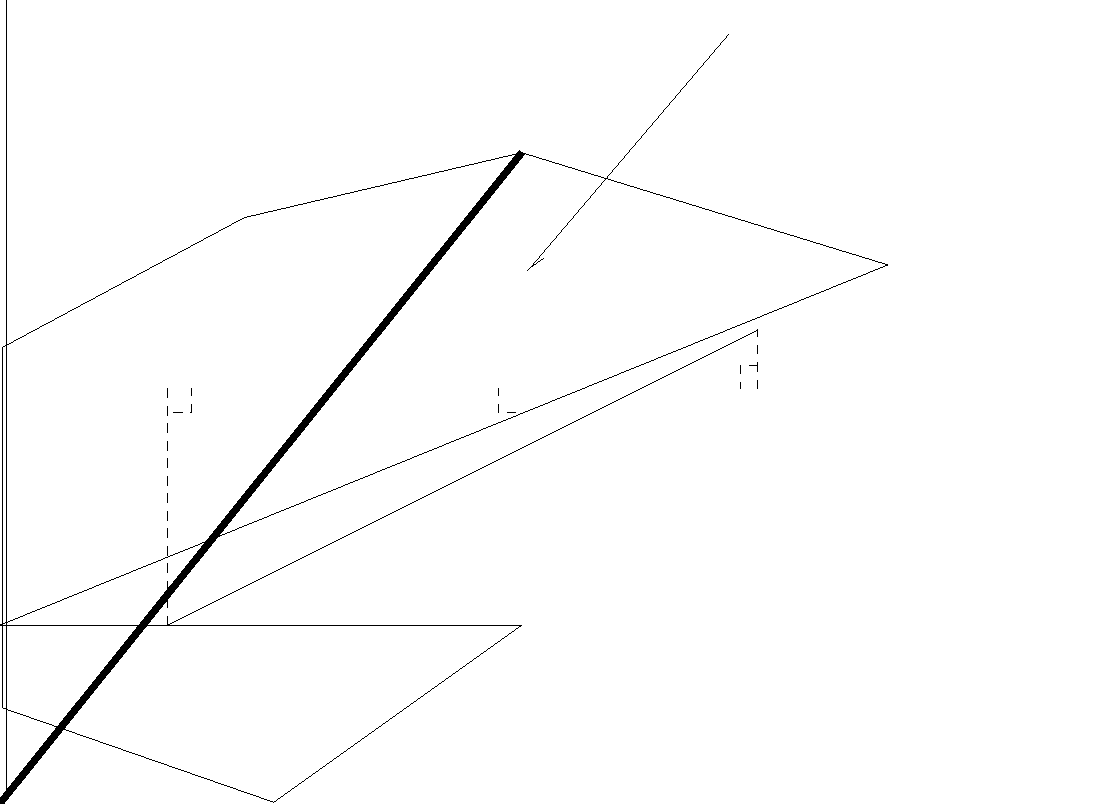
\includegraphics[width=0.4\textwidth]{facette}
} \,
\subfigure[Boundary face]{
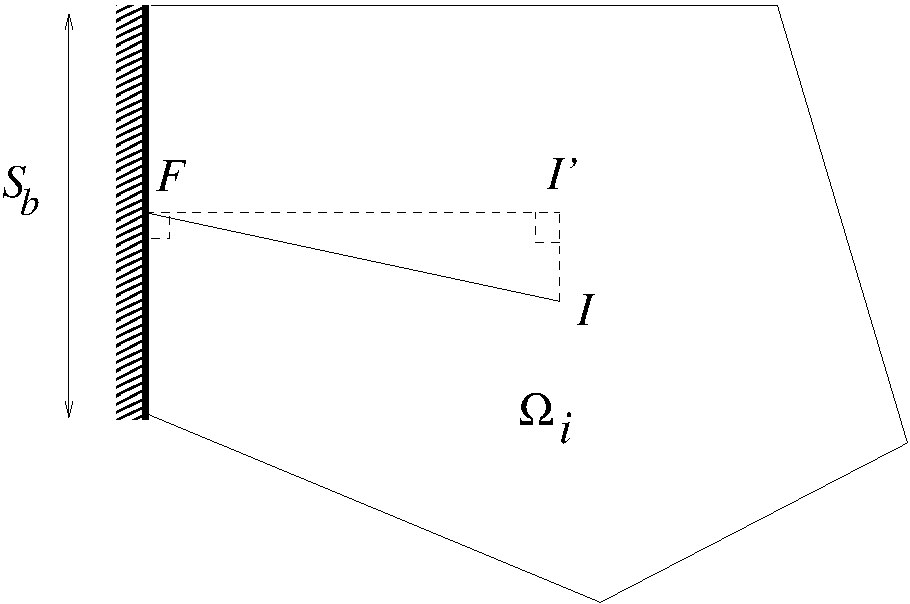
\includegraphics[width=0.4\textwidth]{facebord}
}
}
\caption{\label{fig:geom_gradrc}
Sketch of geometrical quantities.
}
\end{figure}

Notations of the geometrical quantities are recalled in \figurename~\ref{fig:geom_gradrc}.
To compute the cell gradient $\grad_{\celli} \varia $ of the scalar field $\varia$ let us
start by its definition:
\begin{equation}
\norm{\vol{\celli}} \grad_{\celli} \varia \equiv  \displaystyle \int_{\vol{\celli}}{\grad \varia \, \dd \vol{} } = \int_{\partial \vol{\celli}} \varia \dd \vect{S}.
\end{equation}


In order to take the mesh non-orthogonality into account, a Taylor series ($1^{st}$-order) of $\grad_{\celli} \varia$ is used as follows:

\begin{equation}\label{eq:compute_gradrc1}
\begin{array}{r c l}
\norm{\vol{\celli}} \grad_{\celli} \varia &  
\equiv & \displaystyle
\int_{\vol{\celli}}{\grad \varia \, \dd \vol{} }
= \sum\limits_{ \fij \in \Facei{\celli}} 
\varia_{\fij}\,{\vect S_{\ij }} 
+\sum\limits_{ \fib \in \Faceb{\celli}} 
\varia_{\fib}\,{\vect S_{\ib }}, \\
&=& \displaystyle
 \sum\limits_{ \fij \in \Facei{\celli}} 
\varia_{\centf}\,{\vect S_{\ij }} 
+\sum\limits_{ \fib \in \Faceb{\celli}} 
\varia_{\centf}\,{\vect S_{\ib }}, \\
&\simeq &  \displaystyle 
\sum\limits_{ \fij \in \Facei{\celli}} \left[ \varia_{\cento}+ \grad_{\cento} \varia \cdot \vect{\cento \centf} \right] \vect{S}_{\ij}+
\sum\limits_{ \fib \in \Faceb{\celli}} \left[ \epsilon_{\delta \varia} A_{\fib} + B_{\fib} \varia_{\ipf} \right] \vect{S}_{\ib} ,\\
 & = &\displaystyle 
\sum\limits_{ \fij \in \Facei{\celli}} 
\left[
\left( \alpha_{\ij} \varia_\centi +
(1 - \alpha_{\ij}) \varia_\centj \right) \right] \vect{S}_{\ij} +
\sum\limits_{ \fij \in \Facei{i}} \left[
\grad_{\fij} \varia  \cdot  \vect{\cento \centf} \right] \vect{S}_{\ij} \\
&+&\displaystyle 
\sum\limits_{ \fib \in \Faceb{\celli}} \left[ \epsilon_{\delta \varia} A_{\fib} + B_{\fib} \varia_{\ipf} \right] \vect{S}_{\ib} .
\end{array}
\end{equation}

The variable $\epsilon_{\delta \varia}$ is set to $0$ for an increment of a variable\footnote{
Then a homogeneous condition has to be imposed.
},
 to $1$ for the variable itself in order to take 
correctly the boundary condition into account.

Using the following $1^{st}$-order in space approximation
\begin{equation}\notag
\left\{\begin{array}{r c l}
\grad_{\fij} \varia & = & \displaystyle \dfrac{1}{2}\left[ \grad_{\centi} \varia + \grad_{\centj} \varia \right],\\
\varia_{\ipf} &= & \varia_{\centi} + \grad_{\centi} \varia \cdot \vect{\centi \centip } .
\end{array}\right .
\end{equation}
Equation \eqref{eq:compute_gradrc1} becomes:
%
\begin{equation*}
\begin{array}{r c l}
\norm{\vol{\celli}} \grad_{\celli} \varia &=&
\displaystyle
\sum\limits_{\fij \in \Facei{\celli}}
\left[\alpha_{\ij} \varia_\celli
+ (1 - \alpha_{\ij}) \varia_\cellj  + \frac{1}{2}  
\left( \grad_\celli \varia +\grad_\cellj \varia\right) \cdot \vect{\cento \centf }  \right] {\vect S_{\ij}}\\
&+& \displaystyle
\sum\limits_{\fib \in \Faceb{\celli}}
\left[ \epsilon_{\delta \varia}A_{\fib} +
B_{\fib} \varia_{\celli} + B_{\fib} \grad_{\celli} \varia \cdot \vect{\centi \centip}
\right] \vect{S}_{\ib}.
\end{array}
\end{equation*}

Bringing $\grad_\celli \varia$ terms all together on the left hand side, we have:
%
\begin{equation}\label{eq:gradrc_recontruit}
\begin{array}{r c l}
\displaystyle
\norm{\vol{\celli}} \grad_{\celli} \varia -
\sum\limits_{ \fij \in \Facei{\celli}} \frac{1}{2} \grad_\celli \varia \cdot \left( \vect{\cento \centf} \otimes \vect{S}_{\ij} \right)-
\sum\limits_{ \fib \in \Faceb{\celli}} B_{\fib} \grad_\celli \varia \cdot \left( \vect{\centi \centip}  \otimes \vect{S}_{\ib} \right)
&=& 
\displaystyle
\sum\limits_{\fij \in \Facei{\celli}}\left[
(\alpha_{\ij} \varia_\celli + (1 - \alpha_{\ij}) \varia_\cellj)\right] \vect{S}_{\ij} \\
&+&
\displaystyle
\sum\limits_{\fij \in \Facei{\celli}} \frac{1}{2} \grad_\cellj \varia \cdot \left( \vect{\cento \centf} \otimes \vect{S}_{\ij} \right) \\
&+&
\displaystyle
\sum\limits_{\fib \in \Faceb{\celli}}\left[ \epsilon_{\delta \varia} A_{\fib} + B_{\fib} \varia_\celli \right] \vect{S}_{\ib}.
\end{array}
\end{equation}

\subsubsection{Without reconstruction}
On an orthogonal mesh, or if chosen, only $0^{th}$-order contributions are considered.
Everything is as if
$\vect{\centi \centip} = \vect{0}$ and $\vect{\cento \centf} = \vect{0}$ in the previous calculation:
\begin{equation}\notag
\begin{array}{r c l}
\norm{\vol{\celli}} \grad_\celli \varia &\equiv & \displaystyle 
\int_{\vol{\celli}} \grad \varia\, \dd \vol{} =\sum\limits_{\fij \in \Facei{\celli}} \varia_{\fij} \vect S_{\ij} + \sum\limits_{\fib \in \Faceb{\celli}} \varia_{\fib} \vect{S}_{\ib}, \\
 &=& \displaystyle
 \sum\limits_{ \fij \in \Facei{\celli}}
 \left[ \alpha_{\ij} \varia_\centi +
(1 - \alpha_{\ij}) \varia_\centj \right] \vect S_{\ij}
+ \sum\limits_{ \fib \in \Faceb{\celli}} \left[ \epsilon_{\delta \varia} A_{\fib} + B_{\fib}\varia_\centi \right] \vect{S}_{\ib},
\end{array}
\end{equation}
hence
\begin{equation}\label{eq:spadis:gradrc_nonrecontruit}
\grad_\celli^{NRec} \varia= \dfrac{1}{\norm{\vol{\celli}}} \left[
  \sum\limits_{\fij \in \Facei{\celli}} \left[\alpha_{\ij} \varia_\centi + (1 - \alpha_{\ij}) \varia_\centj) \right] \vect S_{\ij} 
+\sum\limits_{\fib \in \Faceb{\celli}}(\epsilon_{\delta \varia} A_{\fib} + B_{\fib} \varia_\centi
) \vect{S}_{\ib} \right].
\end{equation}

\begin{remark}
The non-reconstructed gradient is denoted by $ \grad_\celli^{NRec} \varia  $, and is then 
very easy to compute thanks to the Equation \eqref{eq:spadis:gradrc_nonrecontruit}.
However, it is neither accurate nor consistent on a non-orthogonal mesh.
\end{remark}

\subsubsection{Handling with reconstruction: iterative process}

In order to solve system (\ref{eq:gradrc_recontruit}), all terms containing $\grad_\celli \varia$ are implicit, whereas 
all terms with $\grad_\cellj \varia$ are explicit, we then use the series $\left( \delta \grad_\celli^k \varia \right)_{k \in \mathbb{N}}$ defined by:
%
\begin{equation}
\left\{\begin{array}{r c l}
\delta \grad_\celli^0 \varia &=& \grad_\celli^{NRec} \varia, \\
\delta \grad_\celli^{k+1} \varia &= &\grad_\celli^{k+1} \varia - \grad_\celli^k \varia ,
\end{array}\right.
\end{equation}
%
and the associated system is:

\begin{equation}\label{eq:gradrc_recontruit_comp2}
\begin{array}{r c l}
\displaystyle
\grad_{\celli}^{k+1} \varia \cdot \left[\norm{\vol{\celli}} \tens{1} - 
\sum\limits_{ \fij \in \Facei{\celli}} \frac{1}{2}  \vect{\cento \centf} \otimes \vect{S}_{\ij} -
\sum\limits_{ \fib \in \Faceb{\celli}} B_{\fib} \vect{\centi \centip}  \otimes \vect{S}_{\ib}  \right]
&=& 
\displaystyle
\sum\limits_{\fij \in \Facei{\celli}}\left[
(\alpha_{\ij} \varia_\celli + (1 - \alpha_{\ij}) \varia_\cellj)\right] \vect{S}_{\ij} \\
&+&
\displaystyle
\sum\limits_{\fij \in \Facei{\celli}} \frac{1}{2} \grad_\cellj^k \varia \cdot \left( \vect{\cento \centf} \otimes \vect{S}_{\ij} \right) \\
&+&
\displaystyle
\sum\limits_{\fib \in \Faceb{\celli}}\left[ \epsilon_{\delta \varia} A_{\fib} + B_{\fib} \varia_\celli \right] \vect{S}_{\ib},
\end{array}
\end{equation}
%
or, as the following relationship stands:
\begin{equation*}
 \grad_\celli^{k+1} \varia = \grad_\celli^k \varia+ \delta \grad_\celli^{k+1} \varia ,
\end{equation*}

\begin{equation}\label{eq:gradrc_recontruit_increment}
\begin{array}{r c l}
\displaystyle
\delta \grad_{\celli}^{k+1} \varia \cdot \left[\norm{\vol{\celli}} \tens{1} - 
\sum\limits_{ \fij \in \Facei{\celli}} \frac{1}{2}  \vect{\cento \centf} \otimes \vect{S}_{\ij} -
\sum\limits_{ \fib \in \Faceb{\celli}} B_{\fib}  \vect{\centi \centip}  \otimes \vect{S}_{\ib}  \right]
&=&
\displaystyle
 -\norm{\vol{\celli}}  \grad_{\celli}^{k} \varia +
\sum\limits_{\fij \in \Facei{\celli}}\left[
(\alpha_{\ij} \varia_\celli + (1 - \alpha_{\ij}) \varia_\cellj)\right] \vect{S}_{\ij} \\
&+&
\displaystyle
\sum\limits_{\fij \in \Facei{\celli}} \frac{1}{2} 
\left(\grad_\celli^k \varia + \grad_\cellj^k \varia \right) \cdot \left( \vect{\cento \centf} \otimes \vect{S}_{\ij} \right) \\
&+&
\displaystyle 
\sum\limits_{\fib \in \Faceb{\celli}}\left[ \epsilon_{\delta \varia} A_{\fib} 
            + B_{\fib} \left( \varia_\celli + \grad_\celli^k \varia \cdot \vect{\centi \centip} \right) \right] \vect{S}_{\ib}.
\end{array}
\end{equation}

The Equation (\ref{eq:gradrc_recontruit_increment}) is a local $3 \times 3$ matrix which unknowns are each of the three components of 
the vector $\delta \grad_\celli^{k+1} \varia$. Finally, for each cell $\celli$ we get:
%
\begin{equation}\label{eq:eq_systeme_matriciel_gradrc}
\underbrace{
\left[\begin{array}{c}
\delta \grad_{\celli ,x}^{k+1} \varia\\
\delta \grad_{\celli ,y}^{k+1} \varia\\ 
\delta \grad_{\celli ,z}^{k+1} \varia
\end{array}\right]
}_{\delta \grad_\celli^{k+1} \varia }
\cdot
\underbrace{
\left[\begin{array}{ccc}
\displaystyle
  C_{\celli , xx}
& C_{\celli , xy}
& C_{\celli , xz}\\
\displaystyle
  C_{\celli , yx}
& C_{\celli , yy}
& C_{\celli , yz}\\
\displaystyle
  C_{\celli , zx}
& C_{\celli , zy}
& C_{\celli , zz}
\end{array}\right]
}_{\tens{C}_{\celli}}
=
\underbrace{
\left[\begin{array}{c}
\displaystyle
R^{k+1}_{\celli ,x}\\
\displaystyle
R^{k+1}_{\celli ,y}\\
\displaystyle
R^{k+1}_{\celli ,z}
\end{array}\right]
}_{\vect{R}^{k+1}_{\celli}} , 
\end{equation}
%
with:
%
\begin{equation}\label{eq:eq_second_membre_gradrc}
\left\{\begin{array}{rcl}
\tens{C}_\celli  &=& 
\displaystyle
\norm{\vol{\celli}} \tens{1} - 
\sum\limits_{ \fij \in \Facei{\celli}} \frac{1}{2}  \vect{\cento \centf} \otimes \vect{S}_{\ij} -
\sum\limits_{ \fib \in \Faceb{\celli}} B_{\fib} \vect{\centi \centip}  \otimes \vect{S}_{\ib} ,\\
\vect{R}^{k+1}_{\celli} &=&
\displaystyle 
 -\norm{\vol{\celli}}  \grad_{\celli}^{k} \varia +
\sum\limits_{\fij \in \Facei{\celli}}\left[
(\alpha_{\ij} \varia_\celli + (1 - \alpha_{\ij}) \varia_\cellj)\right] \vect{S}_{\ij} \\
&+& \displaystyle
\sum\limits_{\fij \in \Facei{\celli}} \frac{1}{2} 
\left(\grad_\celli^k \varia + \grad_\cellj^k \varia \right) \cdot \left( \vect{\cento \centf} \otimes \vect{S}_{\ij} \right) \\
&+& \displaystyle 
\sum\limits_{\fib \in \Faceb{\celli}}\left[ \epsilon_{\delta \varia} A_{\fib} 
+ B_{\fib} \left( \varia_\celli + \grad_\celli^k \varia \cdot \vect{\centi \centip} \right)  \right] \vect{S}_{\ib} .
\end{array}\right.
\end{equation}

The invert of the matrix $\tens{C}_{\celli}$ is used to compute $\left( \delta \grad_\celli^{k+1} \varia \right)$ 
and so $\left( \grad^{k+1}_{\celli} \varia \right)$. The iterative process stops as soon as the Euclidean norm of the right-hand-side $\vect{R}^{k+1}_{\celli}$ tends toward zero (\emph{i.e.} when the Euclidean norm
of $\left( \delta \grad^{k}_{\celli} \varia \right)$ tends to zero) or when the number of iterations reaches the maximal number of iterations.

%-------------------------------------------------------------------------------
\subsection{Standard method: iterative process for vectorial fields}\label{sec:spadis:iteratif_gradient_vectors}
In this section, the adaptation of the calculation presented in \S~\ref{sec:spadis:iteratif_gradient} is adapted to 
vectorial fields. Some minor modifications are required, especially for the boundary condition treatment, but the core of the 
formulae are the very similar. The notations of the geometrical quantities are recalled in \figurename~\ref{fig:geom_gradrc}.

The definition of $\gradt_{\celli} \variav $ reads:
\begin{equation}
\norm{\vol{\celli}} \gradt_{\celli} \variav \equiv  \displaystyle \int_{\vol{\celli}}{\gradt \, \variav \, \dd \vol{} } = \int_{\partial \vol{\celli}} \variav \otimes \dd \vect{S}.
\end{equation}

The same Taylor series as \eqref{eq:compute_gradrc1} of $\gradt_{\celli} \variav$ is used:

\begin{equation}\label{eq:compute_gradrv1}
\begin{array}{r c l}
\norm{\vol{\celli}} \gradt_{\celli} \variav &  
\equiv & \displaystyle
\int_{\vol{\celli}}{\gradt \, \variav \, \dd \vol{} }
= \sum\limits_{ \fij \in \Facei{\celli}} 
\variav_{\fij} \otimes {\vect S_{\ij }} 
+\sum\limits_{ \fib \in \Faceb{\celli}} 
\variav_{\fib} \otimes {\vect S_{\ib }}, \\
&=& \displaystyle
 \sum\limits_{ \fij \in \Facei{\celli}} 
\variav_{\centf} \otimes {\vect S_{\ij }} 
+\sum\limits_{ \fib \in \Faceb{\celli}} 
\variav_{\centf} \otimes {\vect S_{\ib }}, \\
&\simeq &  \displaystyle 
\sum\limits_{ \fij \in \Facei{\celli}} \left[ \variav_{\cento}+ \gradt_{\cento} \variav \cdot \vect{\cento \centf} \right] \otimes \vect{S}_{\ij}+
\sum\limits_{ \fib \in \Faceb{\celli}} \left[ \epsilon_{\delta \variav} \vect{A}_{\fib} + \tens{B}_{\fib} \cdot \variav_{\ipf} \right] \otimes\vect{S}_{\ib} ,\\
 & = &\displaystyle 
\sum\limits_{ \fij \in \Facei{\celli}} 
\left[
\left( \alpha_{\ij} \variav_\centi +
(1 - \alpha_{\ij}) \variav_\centj \right) \right] \otimes \vect{S}_{\ij} +
\sum\limits_{ \fij \in \Facei{i}} \left[
\gradt_{\fij} \variav  \cdot  \vect{\cento \centf} \right] \otimes \vect{S}_{\ij} \\
&+&\displaystyle 
\sum\limits_{ \fib \in \Faceb{\celli}} \left[ \epsilon_{\delta \variav} \vect{A}_{\fib} + \tens{B}_{\fib} \cdot \variav_{\ipf} \right] \otimes \vect{S}_{\ib} .
\end{array}
\end{equation}

Once again, the variable $\epsilon_{\delta \variav}$ is set to $0$ for an increment of a variable,
 to $1$ for the variable itself in order to take 
correctly the boundary condition into account.

The same $1^{st}$-order in space approximation as in the scalar gradient calculation is used:
\begin{equation*}
\left\{\begin{array}{r c l}
\gradt_{\fij} \variav & = & \displaystyle \dfrac{1}{2}\left[ \gradt_{\centi} \variav + \gradt_{\centj} \variav \right],\\
\variav_{\ipf} &= & \variav_{\centi} + \gradt_{\centi} \variav \cdot \vect{\centi \centip } .
\end{array}\right .
\end{equation*}
Equation \eqref{eq:compute_gradrv1} becomes:
%
\begin{equation*}
\begin{array}{r c l}
\norm{\vol{\celli}} \gradt_{\celli} \variav &=&
\displaystyle
\sum\limits_{\fij \in \Facei{\celli}}
\left[\alpha_{\ij} \variav_\celli
+ (1 - \alpha_{\ij}) \variav_\cellj  + \frac{1}{2}  
\left( \gradt_\celli \variav +\gradt_\cellj \variav \right) \cdot \vect{\cento \centf }  \right] \otimes {\vect S_{\ij}}\\
&+& \displaystyle
\sum\limits_{\fib \in \Faceb{\celli}}
\left[ \epsilon_{\delta \variav}\vect{A}_{\fib} +
\tens{B}_{\fib} \cdot \variav_{\celli} + \tens{B}_{\fib} \cdot \left( \gradt_{\celli} \variav \cdot \vect{\centi \centip} \right)
\right] \otimes \vect{S}_{\ib}.
\end{array}
\end{equation*}

Note that, there is no simple possibility here to bring 
 $\gradt_\celli \variav$ terms all together on the left hand side, because the term 
 $ \tens{B}_{\fib} \cdot \left( \gradt_{\celli} \variav \right) \cdot \left( \vect{\centi \centip} 
\otimes \vect{S}_{\ib} \right)$ cannot be factorised easily, and thus will be explicit:
%
\begin{equation}\label{eq:gradrv_recontruit}
\begin{array}{r c l}
\displaystyle
\norm{\vol{\celli}} \gradt_{\celli} \variav -
\sum\limits_{ \fij \in \Facei{\celli}} \frac{1}{2} \gradt_\celli \variav \cdot \left( \vect{\cento \centf} \otimes \vect{S}_{\ij} \right)
&=& 
\displaystyle
\sum\limits_{\fij \in \Facei{\celli}}\left[
(\alpha_{\ij} \variav_\celli + (1 - \alpha_{\ij}) \variav_\cellj)\right] \otimes \vect{S}_{\ij} \\
&+&
\displaystyle
\sum\limits_{\fij \in \Facei{\celli}} \frac{1}{2} \gradt_\cellj \variav \cdot \left( \vect{\cento \centf} \otimes \vect{S}_{\ij} \right) \\
&+&
\displaystyle
\sum\limits_{\fib \in \Faceb{\celli}}\left[ \epsilon_{\delta \variav} \vect{A}_{\fib} + \tens{B}_{\fib} \cdot \variav_\celli \right] \otimes \vect{S}_{\ib}
+
\sum\limits_{ \fib \in \Faceb{\celli}} \tens{B}_{\fib} \gradt_\celli \variav \cdot \left( \vect{\centi \centip}  \otimes \vect{S}_{\ib} \right)
.
\end{array}
\end{equation}

\subsubsection{Without reconstruction}
Without reconstruction, the vectorial gradient reads:
\begin{equation}\label{eq:spadis:gradrv_nonrecontruit}
\gradt_\celli^{NRec} \variav= \dfrac{1}{\norm{\vol{\celli}}} \left[
  \sum\limits_{\fij \in \Facei{\celli}} \left[\alpha_{\ij} \variav_\centi + (1 - \alpha_{\ij}) \variav_\centj) \right] \otimes \vect S_{\ij} 
+\sum\limits_{\fib \in \Faceb{\celli}}(\epsilon_{\delta \variav} \vect{A}_{\fib} + \tens{B}_{\fib} \cdot \varia_\centi
)\otimes  \vect{S}_{\ib} \right].
\end{equation}

\subsubsection{Handling with reconstruction: iterative process}

The series $\left( \delta \gradt_\celli^k \variav \right)_{k \in \mathbb{N}}$ is defined by:
%
\begin{equation}
\left\{\begin{array}{r c l}
\delta \gradt_\celli^0 \variav &=& \gradt_\celli^{NRec} \variav, \\
\delta \gradt_\celli^{k+1} \variav &= &\gradt_\celli^{k+1} \variav - \gradt_\celli^k \variav ,
\end{array}\right.
\end{equation}

A system similar to Equation \eqref{eq:gradrc_recontruit_increment} is obtained 
for each cell $\celli$
%
\begin{equation}\label{eq:eq_systeme_matriciel_gradrv}
\delta \gradt_\celli^{k+1} \variav 
\cdot
\tens{C}_{\celli}
=
\tens{R}^{k+1}_{\celli} 
\end{equation}
%
with:
%
\begin{equation}\label{eq:eq_second_membre_gradrv}
\left\{\begin{array}{rcl}
\tens{C}_\celli  &=& 
\displaystyle
 \tens{1} -
\dfrac{1}{\norm{\vol{\celli}}}\sum\limits_{ \fij \in \Facei{\celli}} \frac{1}{2}  \vect{\cento \centf} \otimes \vect{S}_{\ij} 
,\\
\tens{R}^{k+1}_{\celli} &=&
\displaystyle 
 -  \grad_{\celli}^{k} \varia 
 + \dfrac{1}{\norm{\vol{\celli}}}
\sum\limits_{\fij \in \Facei{\celli}}\left[
(\alpha_{\ij} \varia_\celli + (1 - \alpha_{\ij}) \varia_\cellj)\right] \vect{S}_{\ij} \\
&+& \displaystyle
 \dfrac{1}{\norm{\vol{\celli}}}
\sum\limits_{\fij \in \Facei{\celli}} \frac{1}{2} 
\left(\grad_\celli^k \varia + \grad_\cellj^k \varia \right) \cdot \left( \vect{\cento \centf} \otimes \vect{S}_{\ij} \right) \\
&+& \displaystyle 
 \dfrac{1}{\norm{\vol{\celli}}}
\sum\limits_{\fib \in \Faceb{\celli}}\left[ \epsilon_{\delta \varia} A_{\fib} 
+ B_{\fib} \left( \varia_\celli + \grad_\celli^k \varia \cdot \vect{\centi \centip} \right)  \right] \vect{S}_{\ib} .
\end{array}\right.
\end{equation}

\begin{remark}
Note that the matrix $\tens{C}_{\celli}$ in \eqref{eq:eq_second_membre_gradrv} is not the same as in \eqref{eq:eq_second_membre_gradrc}. First of all,
there is no boundary term and thus its invert has not to be recomputed at each iteration (except if the mesh is not modified). This matrix thus  only
measure the quality of the mesh (if the mesh is orthogonal, $\tens{C}_{\celli} = \tens{1}$ for all cells).
Secondly, this matrix is dimensionless, whereas in \eqref{eq:eq_second_membre_gradrc} $\tens{C}_\celli$ has the dimension of a volume. This choice has 
been motivated to minimize truncature errors.
\end{remark}

%-------------------------------------------------------------------------------
\subsection{Least-square method}\label{sec:spadis:least_square_gradient}
%
Notations of the geometrical quantities are recalled in \figurename~\ref{fig:geom_gradrc}.
The aim of the present algorithm is to compute the cell gradient $\grad_{\celli} \varia $ of the scalar field $\varia$
using a least square method. 
The idea is to evaluate the gradient of the variable at the cell faces using the value of the gradient at the cell centres.
The method is supposed to be not as robust as the \emph{iterative} process presented in \S~\ref{sec:spadis:iteratif_gradient}, 
but much more efficient.

Let introduce $\grad_\fij \varia \cdot \vect{d}_\ij$  an estimation at the internal face $\fij$
of the gradient projected in the direction $\vect{d}_{ij}$ (which will be chosen afterwards).
Let also define the analogous quantity for boundary faces $\fib$: $\grad_\fib \varia \cdot \vect{d}_\ib$
 ($\vect{d}_\ib$ will also be chosen afterwards).

The goal would be to find $\grad_{\celli} \varia $ such that, for all faces
the following relationships hold:
\begin{equation}
\left\{\begin{array}{r c l}
\grad_{\celli} \varia  \cdot \vect{d}_\ij &=& \grad_\fij \varia \cdot \vect{d}_\ij , \\
\grad_{\celli} \varia  \cdot \vect{d}_\ib &=& \grad_\fib \varia \cdot \vect{d}_\ib .
\end{array}\right.
\end{equation}

The previous equality is generally not reachable for all the faces, so the 
problem is reformulated as the minimisation of the $\mathcal{F}_\celli$ function: 
%
\begin{equation}\label{eq:spadis:gradmc_function}
\mathcal{F}_\celli
\left( \variav \right) =
\dfrac{1}{2}\sum\limits_{\cellj \in \Neigh{\celli}  }\left[
 \variav   \cdot \vect{d}_\ij  -  \grad_{\fij} \varia   \cdot \vect{d}_\ij 
\right]^2+
\dfrac{1}{2}\sum\limits_{ \fib \in \Faceb{\celli}}\left[
 \variav   \cdot \vect{d}_\ib  -  \grad_{\fib} \varia   \cdot \vect{d}_\ib
\right]^2,
\end{equation}
where $\cellj \in \Neigh{\celli} $ is the neighbouring of the cell $\celli$. By default, the neighbouring is composed of
cells which share at least a face with $\celli$. But \emph{extended} neighbouring can be used. 

To minimize $\mathcal{F}_\celli$, derivatives with respect to the components of the 
vector $\variav  $ are computed, the resulting system is solved and $\grad_\celli \varia$ is defined 
as $\variav_{\min}$ such that $\mathcal{F}_\celli \left( \variav_{\min}\right)$ is minimum.

In order to solve the systems for each cell $\celli$ separately from one to an other,
vectors $\vect{d}_\ij$ and $\vect{d}_\ib$ are chosen so that the quantities 
$\grad_{\fij} \varia   \cdot \vect{d}_\ij $ and $\grad_{\fib} \varia   \cdot \vect{d}_\ib $
do not depend on neighbouring  cell gradients  $\grad_{\cellj} \varia $.
The following choice makes it possible:
\begin{equation}\label{eq:spadis:gradmc_scalar_d_choice}
\begin{array}{r c l}
\vect{d}_\ij &=& \dfrac{\vect{\centi \centj}}{\norm{\vect{\centi \centj}}}, \\
\vect{d}_\ib &=& \dfrac{\vect{\centip \centf}}{\norm{\vect{\centip \centf}}}= \vect{n}_\ib .
\end{array}
\end{equation}

Thus, for internal faces $\fij$, $\vect{d}_\ij$ is the normalized vector joining 
the centres $\centi$ and $\centj$ oriented from cell $\celli$ to $\cellj$.
The quantity  $\grad_{\fij} \varia   \cdot \vect{d}_\ij$ is given by:
\begin{equation}
\grad_{\fij} \varia   \cdot \vect{d}_\ij =\dfrac{\varia_\cellj - \varia_\celli }{\norm{\vect{\centi \centj}}}.
\end{equation}

For boundary faces, the choice $\vect{d}_\ib$ to be the outward normal implies:
\begin{equation}
\grad_{\fib} \varia   \cdot \vect{d}_\ib =\dfrac{\varia_\fib - \varia_\centip }{\norm{\vect{\centip \centf}}},
\end{equation}
where $\varia_\fib$ is expressed thanks to the boundary conditions (see \chaptername~\ref{chapter:bndcnd}) and 
the value $\varia_\centip $ is given by formula \eqref{eq:spadis:reconstruction_ip_jp} recalled hereafter:
%
\begin{equation}\label{eq:spadis:gradmc_bound_value}
\left\{\begin{array}{r c l}
\varia_\centip &=&\varia_\celli +\grad_\celli \varia \cdot \vect{\centi \centip}\\
\varia_\fib &=& A^g_\fib +B^g_\fib \varia_\centip = A^g_\fib +B^g_\fib \left( \varia_\celli +  \grad_\celli \varia \cdot \vect{\centi \centip} \right)
\end{array}\right.
\end{equation}

Eventually we get:
\begin{equation}\label{eq:spadis:gradmc_bound_gradient}
\grad_{\fib} \varia   \cdot \vect{d}_\ib =
\dfrac{  
A^g_\fib +\left(B^g_\fib -1 \right) \left( \varia_\celli +  \grad_\celli \varia \cdot \vect{\centi \centip} \right) 
}{
\norm{\vect{\centip \centf}}
},
\end{equation}

Equation \eqref{eq:spadis:gradmc_bound_gradient} makes appear a term in $\grad_\celli \varia$ 
and thus should be injected into Equation
\eqref{eq:spadis:gradmc_function} before deriving it. Thus \eqref{eq:spadis:gradmc_function} becomes:
\begin{equation}\label{eq:spadis:gradmc_function2}
\begin{array}{r c l}
\mathcal{F}_\celli
\left( \variav \right)& =&
\displaystyle
\dfrac{1}{2}\sum\limits_{ \cellj \in \Neigh{\celli} }\left[
\variav   \cdot \vect{d}_\ij  -  \grad_{\fij} \varia   \cdot \vect{d}_\ij 
\right]^2 \\
&+&
\displaystyle
\dfrac{1}{2}\sum\limits_{ \fib \in \Faceb{\celli}}\left[
  \variav   \cdot  
  \left( \vect{d}_\ib -  \dfrac{B^g_\fib -1 }{\norm{\vect{\centip \centf}}} \vect{\centi \centip} \right) 
-
\dfrac{  
A^g_\fib +\left(B^g_\fib -1 \right) \varia_\celli 
}{
\norm{\vect{\centip \centf}}
}
\right]^2.
\end{array}
\end{equation}


Then we cancel the derivatives of 
$\mathcal{F}_\celli \left( \variav \right)$ with respect to the $ \variav$ components:

\begin{equation}\label{eq:spadis:gradmc_function_derivative}
\begin{array}{r c l}
\der{\mathcal{F}_\celli}{\variav }
\left( \variav \right)& =&
\displaystyle
\sum\limits_{ \cellj \in \Neigh{\celli} }\left[
\left(\variav   \cdot \vect{d}_\ij \right) \vect{d}_\ij  
-  \left(\grad_{\fij} \varia   \cdot \vect{d}_\ij \right)  \vect{d}_\ij
\right] \\
&+&
\displaystyle
\sum\limits_{ \fib \in \Faceb{\celli}}\left[
  \left( \variav   \cdot  
  \left( \vect{d}_\ib -  \dfrac{B^g_\fib -1 }{\norm{\vect{\centip \centf}}} \vect{\centi \centip} \right) \right)
  \left( \vect{d}_\ib -  \dfrac{B^g_\fib -1 }{\norm{\vect{\centip \centf}}} \vect{\centi \centip} \right)
-
\dfrac{  
A^g_\fib +\left(B^g_\fib -1 \right) \varia_\celli 
}{
\norm{\vect{\centip \centf}}
}
\left( \vect{d}_\ib -  \dfrac{B^g_\fib -1 }{\norm{\vect{\centip \centf}}} \vect{\centi \centip} \right)
\right].
\end{array}
\end{equation}


A $3\times 3$ system for each cell $\celli$ 
is got by writing  $\der{\mathcal{F}_\celli}{\variav }
\left( \grad_\celli \varia \right)= \vect{0}$:
%
\begin{equation}\label{eq:spadis:gradmc_matrix}
\grad_\celli \varia \cdot \tens{C}_\celli = \vect{R}_\celli ,
\end{equation}
with
%
\begin{equation}
\left\{
\begin{array}{r c l}
\tens{C}_\celli &=&
\displaystyle
 \sum\limits_{\cellj \in \Neigh{\celli} } 
 \vect{d}_\ij \otimes \vect{d}_\ij
+
\sum\limits_{\fib \in \Faceb{\celli}}
\left( \vect{d}_\ib -\dfrac{ B^g_\fib -1}{\norm{\vect{\centip \centf}}}  \vect{\centi \centip } \right)
\otimes
\left( \vect{d}_\ib -\dfrac{ B^g_\fib -1}{\norm{\vect{\centip \centf}}}  \vect{\centi \centip } \right),
\\
\vect{R}_\celli &=&
\displaystyle
\sum\limits_{ \cellj \in \Neigh{\celli} }
\left( \grad_{\fij} \varia   \cdot \vect{d}_\ij \right) \vect{d}_\ij 
+
\sum\limits_{ \fib \in \Faceb{\celli}}
\dfrac{  
A^g_\fib +\left(B^g_\fib -1 \right) \varia_\celli 
}{
\norm{\vect{\centip \centf}}
} 
\left( \vect{d}_\ib -  \dfrac{B^g_\fib -1 }{\norm{\vect{\centip \centf}}} \vect{\centi \centip} \right),
\end{array}\right.
\end{equation}
%
using \eqref{eq:spadis:gradmc_scalar_d_choice} this gives:
\begin{equation}
\left\lbrace
\begin{array}{r c l}
\tens{C}_\celli &=&
\displaystyle
 \sum\limits_{\cellj \in \Neigh{\celli} } 
 \dfrac{\vect{\centi \centj} \otimes \vect{\centi \centj}}{\norm{\vect{\centi \centj}}^2}
 +
\sum\limits_{\fib \in \Faceb{\celli}}
\left( \vect{n}_\ib -\dfrac{ B^g_\fib -1}{\norm{\vect{\centip \centf}}}  \vect{\centi \centip } \right)
\otimes
\left( \vect{n}_\ib -\dfrac{ B^g_\fib -1}{\norm{\vect{\centip \centf}}}  \vect{\centi \centip } \right),
\\
\vect{R}_\celli &=&
\displaystyle
\sum\limits_{ \cellj \in \Neigh{\celli} }
\left( \varia_\cellj - \varia_\celli  \right) \dfrac{ \vect{\centi \centj}}{\norm{\vect{\centi \centj}}^2} 
+
\sum\limits_{ \fib \in \Faceb{\celli}}
\dfrac{  
A^g_\fib +\left(B^g_\fib -1 \right) \varia_\celli 
}{
\norm{\vect{\centip \centf}}
} 
\left( \vect{n}_\ib -  \dfrac{B^g_\fib -1 }{\norm{\vect{\centip \centf}}} \vect{\centi \centip} \right).
\end{array}\right.
\end{equation}

\begin{remark}
\begin{enumerate}[ label=\roman{*}/, ref=(\roman{*})]
\item Note that the $3\times3$ $\tens{C}_\celli$ tensor is symmetric.
\item For cells $\celli$ having at least a boundary face $\fib$, the tensor $\tens{C}_\celli$ must be recomputed at each time step,
for the other, the tensor $\tens{C}_\celli$ only have to be recomputed when the mesh is updated (in ALE for instance).
\item If the user chooses not to reconstruct the gradients (which introduces a lack of consistency on non-orthogonal meshes),
then the gradient is computed thanks to formula \eqref{eq:spadis:gradrc_nonrecontruit}.
\item For highly non-orthogonal meshes, an extended support\footnote{
the support is the set of neighbouring cells used in the cell gradient computation.
} can be used (see different support in \figurename~\ref{fig:spadis:gradmc_support}) and can drastically improve the results when using tetrahedral meshes. 
\end{enumerate}
\end{remark}

\begin{figure}[!htp]
\centerline{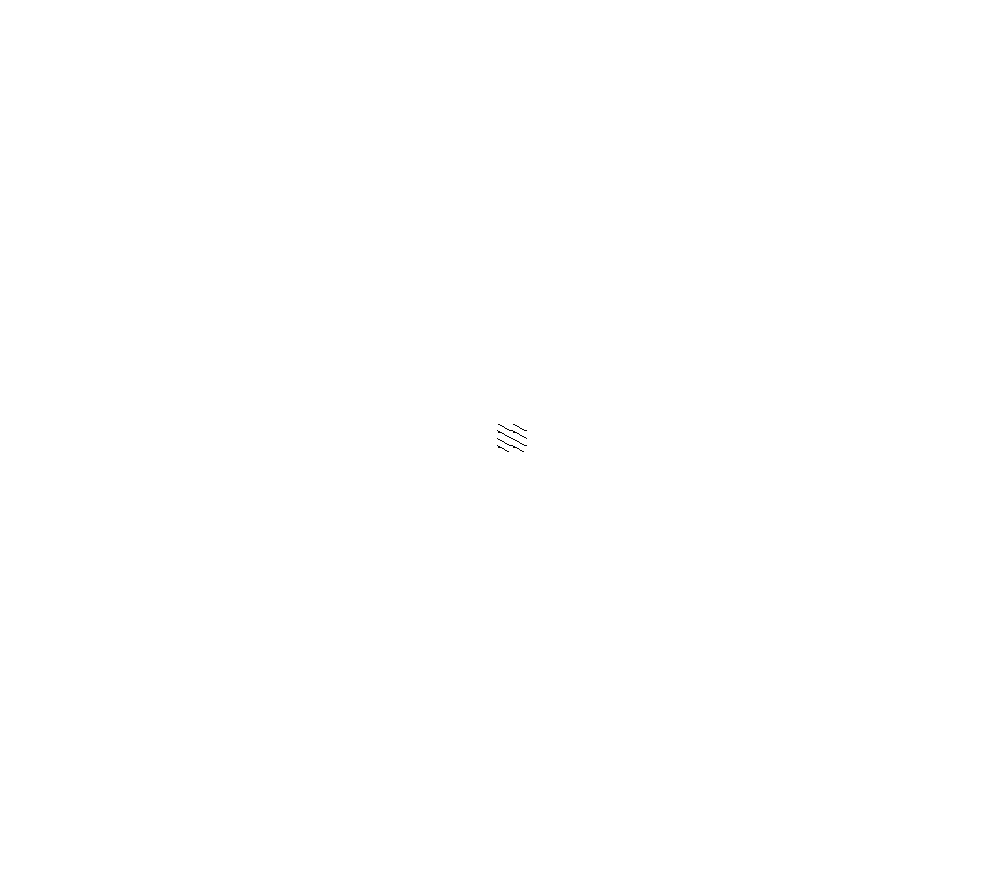
\includegraphics[height=8cm]{support}}
\caption{Available supports for computing the gradient with the least square method.\label{fig:spadis:gradmc_support}}
\end{figure}


%-------------------------------------------------------------------------------
\subsection{Least-square method for vectorial fields}\label{sec:spadis:least_square_gradient_vectors}
%
In this section, the adaptation of the calculation presented in \S~\ref{sec:spadis:least_square_gradient} is adapted to 
vectorial fields. Some minor modifications are required, especially for the boundary condition treatment, but the core of the 
formulae are the very similar. The notations of the geometrical quantities are recalled in \figurename~\ref{fig:geom_gradrc}.

The functional to be minimized is defined by
%
\begin{equation}\label{eq:spadis:gradmv_function}
\mathcal{F}_\celli
\left( \variat \right) =
\dfrac{1}{2}\sum\limits_{\cellj \in \Neigh{\celli}  }
\norm{
 \variat   \cdot \vect{d}_\ij  -  \gradt_{\fij} \variav   \cdot \vect{d}_\ij 
}^2+
\dfrac{1}{2}\sum\limits_{ \fib \in \Faceb{\celli}}
\norm{
 \variat   \cdot \vect{d}_\ib  -  \gradt_{\fib} \variav   \cdot \vect{d}_\ib
}^2,
\end{equation}

To minimize $\mathcal{F}_\celli$, derivatives with respect to the components of the 
vector $\variat  $ are computed, the resulting system is solved and $\gradt_\celli \variav$ is defined 
as $\variat_{\min}$ such that $\mathcal{F}_\celli \left( \variat_{\min}\right)$ is minimum.

In order to obtain a simple system, the same choice as in \eqref{eq:spadis:gradmc_scalar_d_choice} is made on $\vect{d}_\ij$.
Concerning $\vect{d}_\ib$, an other choice ensuring that $\grad_{\fib} \varia   \cdot \vect{d}_\ib $ does not
depend on $\grad_{\celli} \varia $ is made:
%
\begin{equation}\label{eq:spadis:gradmv_scalar_d_choice}
\begin{array}{r c l}
\vect{d}_\ij &=& \dfrac{\vect{\centi \centj}}{\norm{\vect{\centi \centj}}}, \\
\vect{d}_\ib &=& \dfrac{\vect{\centi \centf}}{\norm{\vect{\centi \centf}}} .
\end{array}
\end{equation}

Thus, for internal faces $\fij$, $\vect{d}_\ij$ is still the normalized vector joining 
the centres $\centi$ and $\centj$ oriented from cell $\celli$ to $\cellj$.
The quantity  $\gradt_{\fij} \variav   \cdot \vect{d}_\ij$ is given by:
\begin{equation}
\gradt_{\fij} \variav   \cdot \vect{d}_\ij =\dfrac{\variav_\cellj - \variav_\celli }{\norm{\vect{\centi \centj}}}.
\end{equation}

For boundary faces, the choice $\vect{d}_\ib$ implies:
\begin{equation}
\gradt_{\fib} \variav   \cdot \vect{d}_\ib =\dfrac{\variav_\fib - \variav_\celli }{\norm{\vect{\centi \centf}}},
\end{equation}
where $\variav_\fib$ is expressed thanks to the boundary conditions (see \chaptername~\ref{chapter:bndcnd}).

Then we cancel the derivatives of 
$\mathcal{F}_\celli \left( \variat \right)$ with respect to the $ \variat$ components:


A $3\times 3$ system for each cell $\celli$ 
is got by writing  $\der{\mathcal{F}_\celli}{\variat }
\left( \gradt_\celli \variav \right)= \tens{0}$:
%
\begin{equation}\label{eq:spadis:gradmv_matrix}
\gradt_\celli \variav \cdot \tens{C}_\celli = \tens{R}_\celli ,
\end{equation}
with
%
\begin{equation}
\left\{
\begin{array}{r c l}
\tens{C}_\celli &=&
\displaystyle
 \sum\limits_{\cellj \in \Neigh{\celli} } 
 \vect{d}_\ij \otimes \vect{d}_\ij
+
\sum\limits_{\fib \in \Faceb{\celli}}
\vect{d}_\ib \otimes  \vect{d}_\ib ,
\\
\tens{R}_\celli &=&
\displaystyle
\sum\limits_{ \cellj \in \Neigh{\celli} }
 \gradt_{\fij} \variav   \cdot \left( \vect{d}_\ij \otimes \vect{d}_\ij \right)
+
\sum\limits_{ \fib \in \Faceb{\celli}}
\dfrac{  
\vect{A}^g_\fib +\left(\tens{B}^g_\fib -\tens{1} \right) \cdot \variav_\celli 
}{
\norm{\vect{\centi \centf}}
} 
\otimes
\vect{d}_\ib .
\end{array}\right.
\end{equation}
%


\begin{remark}
Note that the $3\times3$ $\tens{C}_\celli$ tensor is  slightly different from \eqref{eq:spadis:gradmc_matrix} and does not depend
 on boundary condition coefficients (and thus does not require re-computation if the mesh is not modified. 
\end{remark}







%-------------------------------------------------------------------------------
\section{Advanced topic}

%-------------------------------------------------------------------------------
\subsection{Rhie \& Chow filter}


%-------------------------------------------------------------------------------
\subsection{Handling of the hydrostatic pressure}

%-------------------------------------------------------------------------------
\subsection{Pressure extrapolation at the boundaries}


